%!TEX root = ../thesis-main.tex

\chapter{Analisi}

\section{Requisiti}

Il progetto si pone due principali obiettivi:
\begin{itemize}
	\item La generazione automatica di pacchetti di installazione multi-piattaforma.
	\item La pubblicazione automatica dei rilasci del software all'interno di repository pubblici selezionati.
\end{itemize}
Un pacchetto software è un insieme di risorse necessarie per eseguire un'applicazione o un servizio su un sistema. Sono usualmente distribuiti all'interno di archivi compressi contenenti meta-dati che ne descrivono la forma e l'utilizzo. La pubblicazione è l'atto di inserire il software in archivi (repository) online con l'intento di consentire l'installazione agli utenti finali. Entrambi i processi devono essere automatizzati e integrati all'interno di una pipeline di integrazione e rilascio continua.

\paragraph{Requisiti funzionali}

Le funzionalità richieste si possono classificare in due gruppi distinti: il primo contiene tutto ciò che concerne l'esperienza dell'utente finale, mentre il secondo descrive le funzionalità dal punto di vista degli sviluppatori e contributori di Alchemist. Di seguito il primo gruppo:
\begin{itemize}
	\item \textbf{Pacchettizzazione}: il simulatore deve essere distribuito in pacchetti \textit{self-contained}, ossia contenenti l'intera applicazione, e più specificatamente nell'ambito \ac{jvm}, integranti un \ac{jre} adibito all'esecuzione.
	\item \textbf{Multi-piattaforma}: Alchemist deve essere installabile sui maggiori sistemi operativi in circolazione come Windows, MacOS e le principali distribuzioni Linux.
	\item \textbf{Plug and play}: l'installazione non deve richiedere configurazioni complesse, l'applicativo deve essere pronto all'uso non appena installato.
\end{itemize}

I requisiti del gruppo successivo sono accumunabili per il loro scopo, vale a dire l'automazione:

\begin{itemize}
	\item \textbf{Automazione dei pacchetti}: la generazione dei pacchetti di installazione deve essere automatica e configurabile.
	\item \textbf{Automazione della distribuzione}: il rilascio di una nuova versione comprende la distribuzione di essa nei repository selezionati e deve essere svolta in modo automatico.
	\item \textbf{Verifica funzionamento}: entrambi i processi descritti precedentemente devono essere corredati da verifiche del loro funzionamento e devono bloccare la procedura di rilascio nell'eventualità siano presenti errori.
\end{itemize}

\paragraph{Requisiti non funzionali}

\begin{itemize}
	\item Trattandosi Alchemist di un software in continuo sviluppo, è auspicabile l'utilizzo degli strumenti già impiegati nel progetto. \\ L'integrazione di nuovi applicativi deve essere eseguita solo se strettamente necessaria.
	\item La pipeline \ac{cicd} ottenuta deve garantire prestazioni in linea con la versione precedente l'intervento di questo progetto.
\end{itemize}

\section{Pacchettizzazione}\label{sec:packaging}

Come si evince dall'analisi svolta, la pacchettizzazione è un requisito fondamentale dell'elaborato. Sino a ora l'applicativo Alchemist era distribuito in file JAR, ossia archivi java compressi contenenti tutte le dipendenze e i relativi \textit{classfiles} necessari all'esecuzione. Quest'approccio molto diffuso porta con sè diverse limitazioni tra cui:
\begin{itemize}
	\item la necessità dell'utente scaricante di avere un \ac{jre} installato nel proprio dispositivo;
	\item il potenziale bisogno di utilizzare un ambiente \ac{jre} specifico e quindi per l'utente di non possedere una versione dell'ambiente compatibile;
	\item la difficoltà di utilizzo per utenti non esperti, abituati a eseguire programmi utilizzando file eseguibili nativi della propria piattaforma.
\end{itemize}
Alcune di queste restrizioni risultano mitigate, tuttavia non in tutte le piattaforme, come Windows, il quale per esempio non fornisce un ambiente java pre-installato. Esistono diversi strumenti di terze parti e non che cercano di far fronte a questo problema, è importante dunque valutare e scegliere lo strumento più opportuno.

\subsection{Soluzioni}

Nell'ottica di semplificare la configurazione di questo processo lo strumento selezionato deve supportare le tre principali piattaforme descritte nei requisiti precedentemente. Tra gli strumenti analizzati due molto differenti si sono distinti, vale a dire: \textit{jpackage}, comando disponibile nel \ac{jdk} dalla versione 14, adibito alla produzione di pacchetti self-contained con \ac{jre} integrata e \textit{GraalVM}, un \ac{jdk} sviluppato da Oracle che fornisce un compilatore \ac{jit} e \ac{aot} per java. 

La modalità \ac{jit} descrive il comportamento normale di ogni \ac{jvm}: il compilatore Java traduce il programma ad alto livello in bytecode, e successivamente la \ac{jvm} converte dinamicamente il bytecode in linguaggio macchina per l'architettura specifica. In contrasto la tecnica \ac{aot} ricorda i linguaggi di programmazione compilati, ovvero la compilazione è statica e avviene prima dell'esecuzione del programma. Il compilatore \ac{aot} chiamato ``Native Image", consente di compilare un programma java (e altri linguaggi di programmazione) ottenendo in output un eseguibile nativo per ogni piattaforma. Quest'ultimo inoltre porta con sè diversi vantaggi come: un minor costo in risorse CPU e memoria, tempi di avvio minori e dimensioni ridotte rispetto un normale programma java distribuito con un \ac{jre}. La compilazione \ac{aot} però ha dei requisiti, uno di questi fondamentale è la \textit{closed world assumption}: ossia ogni parte di codice raggiungibile in esecuzione lo deve essere anche in fase di build. Ciò accade perché native image svolge un analisi statica del codice, pertanto alcune funzionalità come la reflection oppure il caricamento dinamico non sono supportate e richiedono una soluzione alternativa.

In contrasto \textit{jpackage} fornisce uno strumento interessante, il quale non richiede modifiche all'applicativo ed è pre-installato in tutti i \ac{jdk} dalla versione 14 e successive. Lo strumento risolve le problematiche esposte inizialmente mediante l'annessione di un \ac{jre} utilizzando \textit{jlink}. Inoltre, produce diverse tipologie di pacchetti per ogni piattaforma ed è completamente controllabile da interfaccia \ac{cli}. Le tipologie di pacchetti generabili sono elencate di seguito:
\begin{itemize}
	\item \textit{exe} e \textit{msi} per Windows;
	\item \textit{rpm} e \textit{deb} per Linux;
	\item \textit{pkg} e \textit{dmg} per MacOs.
\end{itemize}
Tuttavia anch'esso presenta dei limiti come: la necessità di essere eseguito sullo stesso sistema operativo dove i pacchetti prodotti sono destinati (lo stesso vale per GraalVM, la \textit{cross compilation} non è supportata) e la produzione di un solo pacchetto per singola esecuzione.

\paragraph{Valutazione finale} Ambedue le soluzioni, seppure differenti concorrono all'obiettivo primario: la distribuzione del software multi-piattaforma. GraalVM fornisce diversi vantaggi prestazionali, ma i requisiti da esso richiesti non sono compatibili con l'architettura del simulatore. D'altro canto jpackage fornisce tutto il necessario per costruire i pacchetti con embed di un \ac{jre} senza la necessità di stravolgere l'architettura del software, e i limiti delineati sono superabili adoperando script o configurazioni specifiche.

\section{Analisi degli strumenti}

Gli strumenti presentati nella sezione \ref{sec:technologies} costituiscono il progetto Alchemist nel suo complesso. Grazie agli script Gradle, il simulatore gestisce in modo efficace i processi di compilazione, generazione della documentazione ed esecuzione delle verifiche del codice. Mentre l'utilizzo della piattaforma Actions fornisce l'infrastruttura necessaria e le API per creare una pipeline di \ac{cicd}. 

\begin{figure}[htb]
	\centering
	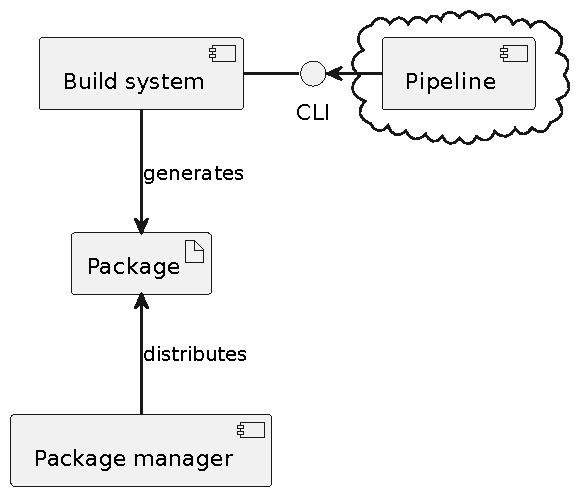
\includegraphics[width=.6\linewidth]{figures/components-diagram.pdf}
	\caption{Diagramma dei componenti che interagiscono nel progetto}
	\label{fig:components-diagram}
\end{figure}

In considerazione dei requisiti posti, la pacchettizzazione risulta un processo di produzione di artefatti ed è perciò necessaria la sua integrazione nel build system. Mediante l'integrazione, si garantisce un corretto ordine di esecuzione rispetto ai diversi processi che il simulatore configura, con l'effetto di minimizzare l'incidenza di errori e assicurando la produzione di pacchetti conformi su qualsiasi sistema operativo in cui Gradle viene eseguito. Contemporaneamente Actions si occupa di offrire l'infrastruttura per automatizzare i processi esposti dal build system. La piattaforma fornisce le funzionalità necessarie a soddisfare i requisiti di automazione posti precedentemente, in particolare mediante: la possibilità di utilizzare macchine virtuali (runner) di tutte e tre i sistemi operativi target, la possibilità di configurare eventi o esecuzioni ricorrenti di processi e tramite la presenza di un'infrastruttura cloud resiliente per l'esecuzione della pipeline. Nel diagramma rappresentato nella \cref{fig:components-diagram}, sono illustrate le interazioni tra gli strumenti descritti. La pipeline, eseguita in un ambiente cloud, utilizza l'interfaccia fornita dal build system per generare il pacchetto di installazione e distribuirlo in modo che sia accessibile tramite i gestori di pacchetti designati.

\subsection{Distribuzione dei pacchetti}

La distribuzione ricopre un ruolo centrale nel processo di rilascio del software. L'obiettivo principale è estendere la disponibilità del simulatore Alchemist attraverso il maggior numero possibile di repository, al fine di permettere a più utenti possibili di installare e utilizzare il software. Nei prossimi paragrafi, verranno presentate due principali piattaforme di distribuzione coinvolte in questo progetto

\paragraph{Arch User Repository} Tra i numerosi fork Linux, Arch occupa una posizione di rilievo nel panorama. Basata sull'architettura x86-64, Arch Linux è stata sviluppata con l'adesione alla filosofia \ac{kiss}. Conosciuta per la sua leggerezza, velocità, e la sua estrema scalabilità, questa distribuzione si distingue per la sua capacità di adattarsi alle esigenze specifiche di ogni utente. Data la sua natura minimalista, l'installazione iniziale non incorpora alcun strumento di configurazione automatica, nessun ambiente desktop e nessun altro strumento necessario all'avvio del sistema. 

Il sistema di gestione dei pacchetti si chiama \textit{pacman} e a differenza dei concorrenti, opera sia a basso che ad alto livello. Un pacchetto non è altro che un file shell script, denominato \textit{PKGBUILD}, contenente le istruzioni necessarie a scaricare i sorgenti e compilarli attraverso un comando: \textit{makepkg}. La linearità dei file PKGBUILD rende la creazione di pacchetti alla portata di qualsiasi utente, difatti Arch supporta l'\textbf{\ac{aur}}, un tratto distintivo di questa distribuzione. Si tratta di un repository di pacchetti in cui qualsiasi utente, anche non sviluppatore, può contribuire. Pertanto, la facilità di accesso e la mancanza di requisiti stringenti danno luce a un ambiente perfetto per la distribuzione del simulatore.

\paragraph{Windows e winget} Un discorso differente vale per Windows, dove fino a poco tempo fa non era previsto alcun package manager ufficiale pre-installato. Gli utenti solitamente installavano software attraverso pacchetti distribuiti in siti web ad-hoc, store non ufficiali o tramite il Microsoft Store. D'altra parte gli sviluppatori, per sfruttare i benefici della gestione a pacchetti, ricorrono a gestori di terze parti. Solamente nel settembre 2020 è stato introdotto ``winget": un package-management system open-source sviluppato da Microsoft, che supporta pacchetti di installazione EXE, MSIX e MSI. Il repository dei pacchetti è accessibile pubblicamente ed è possibile mediante richieste di contribuzione e previa approvazione, pubblicare pacchetti all'interno di esso. \\

Poiché Windows e MacOs sono sistemi operativi closed-source, essi non richiedono particolari attenzioni in quanto le tipologie di pacchetti generabili da jpackage sono sufficienti e ufficialmente supportate. Linux al contrario è notevolmente frammentato, ogni distribuzione può adottare uno dei tanti sistemi di gestione dei pacchetti o introdurne uno nuovo. Purtroppo, non esistono statistiche ufficiali riguardo la diffusione delle distribuzioni, molte di esse si basano su stime o dati non attendibili. D'altra parte, analizzando i pacchetti generabili da jpackage possiamo trarre delle conclusioni.
\begin{itemize}
	\item \textbf{RPM} significa "RedHat Package Manager" ed è un formato di pacchetti progettato per RedHat e le distribuzioni derivate. 
	\item \textbf{DEB} è l'abbreviazione di ``Debian packages", è una tipologia di pacchetto supportata da Debian e le distribuzioni derivate. Secondo distrowatch\footnote{https://distrowatch.com/}, Debian Linux presenta più di 400 distribuzioni derivate e più di 120 di queste sono attualmente attive.
\end{itemize}
È evidente come le due tipologie coprano un ampio spettro nel panorama Linux. Inoltre, esse sono supportate dallo script PKGBUILD nativamente, poiché il comando \textit{makepkg} supporta l'estrazione di questi pacchetti in modo autonomo. 

In conclusione, jpackage fornisce tutto il necessario per supportare in modo completo le piattaforme closed-source disponibili. Riguardo a Linux, i due tipi di pacchetti descritti svolgono un ruolo fondamentale nell'integrare diverse distribuzioni e rendere il software compatibile con l'\ac{aur}, contribuendo così ad ampliare la sua compatibilità nel vasto panorama delle distribuzioni Linux.
